\chapter{Methodology}
\label{chapter:Methods}

This chapter adds transparency to the research process. The main research question is divided in sub-questions (Section \ref{section:sub_questions}). Research methodologies are defined in correspondence with these sub-questions (Section  \ref{section:Methods_fieldwork} - \ref{section:Theory_yields}). The research definitions, theoretics and model compositions are included here. Collectively, the methodologies are a framework to provide the research with answers.

\section{Research sub-questions}
\label{section:sub_questions}

The main research question can be solved in consecutive parts. Besides the main research question, three sub-question are stated that have to be answered: \\
 
\textbf{How can improvements of Aquifer Storage and Recovery (ASR) systems be more beneficial for the availability and sustainable use of groundwater in northern Ghana small-scale agriculture?}

\begin{itemize}
\item{\textit{Which (range of) values for transmissivity ($T$) and storativity ($S$) can be obtained from the data analysis of pumping tests applied at multiple study sites in northern Ghana?}
\smallskip \\
It might seem trivial, but the functioning of an ASR system is dependent on its surroundings. The locally applicable soil parameters ($T$ and $S$) have to be determined for the research follow-ups. The desired information is obtained by the application of site-specific measurements within northern Ghana. The Fieldwork set-up strategies as well as the approaches in data analysis are included in the methodology (Section \ref{section:Methods_fieldwork}). The answers to the sub-question are generated in Chapter \ref{chapter:Fieldwork_data_analysis}.} 
\end{itemize} 

\begin{itemize} 
%\item{\textit{How and to what extent can ASR system improvements gain groundwater discharge rates, while maintaining sustainable use of natural resources?}}
%\item{\textit{How and to what extent can northern Ghana smallholder farmers improve ASR systems; increase groundwater discharge while sustainability is maintained?}}
%\item{\textit{How and to what extent can ASR system improvements be beneficial for northern Ghana smallholder framers, while sustainability is maintained?}}
\item{\textit{How and to what extent can improvements of an ASR system increase the water supply to northern Ghana smallholder framers, while sustainability is maintained?}
\smallskip \\
For northern Ghana smallholder farmers this question is key, but the answer to it is rather challenging. The terms 'how' (types of improvement) and 'to what extent' (limit of sustainability) need further specifications. In order to judge the improvements of the ASR system, comparison material is required. A northern Ghana synthetic base model is defined as reference (Section \ref{section:test_problem_def}). The outcomes of the (improved) system simulations are elaborated in Chapter \ref{chapter:model_scenarios}.}
\end{itemize}

\begin{itemize}
%\item{\textit{What is in potential the magnitude of a synthetic ASR system on agricultural and financial yields?}}
%\item{\textit{Which order in agricultural and financial yield can potentially be associated with a synthetic ASR system in northern Ghana?}}
%\item{\textit{What order of yield size can potentially be associated with a northern Ghana synthetic ASR system?}}
%\item{\textit{What can potentially be the magnitude of an northern Ghana synthetic ASR system on agricultural and financial yield?}
\item{\textit{With what potential levels of (financial) yield can a northern Ghana synthetic ASR system be associated?}
\smallskip \\
The synthetic ASR system and system improvements are generally expressed in water volumes. Transformations towards agricultural and financial yields are desired to give more insight/perspective to the ASR system magnitude. Theoretics on pumping costs and crop-specific yield are defined in the methodology (Section \ref{section:Theory_yields}). The systems feasibility (financially) is roughly addressed in chapter \ref{chapter:yield}.}
\end{itemize}

The subsequent sections (Section \ref{section:Methods_fieldwork} - \ref{section:Theory_yields}) contain the research methodologies. While the actual answers to the sub-questions are included in the successive research chapters (Chapter \ref{chapter:Fieldwork_data_analysis} - \ref{chapter:yield}). \\

\section{Methods - Fieldwork set-up \& analysis}
\label{section:Methods_fieldwork}
The first research steps are aimed at the collection of fieldwork data. The applied processes, from nil to fieldwork data to geohydrological parameter values, are included in this section. A total of five northern Ghana study sites (Chapter \ref{section:research_locations}) are subjected to the methods described here. The results can be found in Chapter \ref{chapter:Fieldwork_data_analysis}. Additional information is included in the Appendices \ref{chapter:Borehole_logsheets} - \ref{chapter:Extense_fieldwork_analysis}.

\subsection{Measurement set-up}
\label{subsection:measurement_structure}
This section accommodates the ins and outs of the research fieldwork set-up. Due to differences in ASR systems encountered, the data collection is designed by a hybrid measurement approach. The stated approach provides research transparency and can be used as input for data (re)production. \\

\textbf{Pump installation} \\
Based on the (2016) original log sheets (Appendix \ref{chapter:Borehole_logsheets}), site-specific borehole depths are known in advance. The fieldwork ASR system inspection showed, borehole depths are decreased over time due to the accumulation of sedimentation. To prevent pump damages and make sure properly functioning is maintained, actual borehole depths are measured before pumping tests are executed. Outcomes of the measurements are taken into account for each individual set-up. To prevent the excessive spread of soil particles, the submersible pump is positioned at least 5 m above the measured bottom. In practice, this resulted in a pump suction depth of approximately 30-35 m.
\bigskip \\
\textbf{Pump discharge \& measurement} \\
A single 100 m hose is directly connected to the outlet of the submersible pump. Based on the pump position (deep inside borehole), a distance of circa 65 m is applied for the horizontal displacement of water. At this distance, water is discharged on the surface.
\\
The head of the hose is equipped with a nozzle to roughly regulate the discharge rate. By the use of this nozzle, discharge rates in the range of 50-75 m$^{3}$/d are obtained during the pumping tests. Rates are measured by the use of a stopwatch and a 50 l bucket. Starting at the moment of pump operation, the duration of filling is measured twice every 15 minutes. The obtained average is used to calculate the time dependent discharge rates. More detailed discharge information can be found in the site-specific fact sheets (Appendix \ref{chapter:fieldworkresults}).
\bigskip \\
\textbf{Groundwater table (GWT) measurement} \\
Groundwater level reductions caused by pumping tests are preferably measured in multiple piëzometers, located at a certain known horizontal distance from the discharge well \citep{Kruseman2000}. In the northern Ghana surroundings, close range monitoring options are absent. Due to a lack of time and/or resources these facilities could not be arranged either. Moreover, the implementation of such facilities do not match research nature. Aim of this research is to collect fieldwork data by the use of minimal resources. The absence of widespread measurement options strengthens this approach. As a consequence, the time dependent GWTs (drawdowns) are measured in the discharge well only. \\
A water tape is used as hand equipment. First of all to determine the initial (static) GWT. Subsequently, the device is applied as a real time indicator of drawdown. During the pumping tests, multiple hand measurements are applied at randomly picked moments to monitor the progress. Gathered data functions as verification and back-up of the pressure sensors (divers), which are normative. \\
Two types of divers (different brands) are used as basic GWT measurement devices. Product specifications show that these divers can respectively measure pressures up to 10 m (Van Essen) and 9 m (In-Situ) water column (Appendix \ref{chapter:fieldwork_set-up}). The northern Ghana regional subsurface is characterized as highly heterogeneous. The pumping test GWT drawdown magnitude is therefore unpredictable. To prevent the occurrence of missing drawdown data, the single borehole is equipped with multiple divers at ascending depths. The water column between the initial static water table and pump position is filled with about four divers, with a mutual distance that meets the divers range specifications. To make sure the divers stay in position they are leashed to a rope which runs from well top to pump. This measurement set-up forms a robust network for the collection of drawdown data (figure~\ref{fig:general}). \\
However, practical circumstance can cause the application of a more simplistic set-up (figure~\ref{fig:simplified}). One can think of a situation in which the pump is already installed and/or will not be removed at the end of the pumping test. In this case, the (rope) attachment of the divers to the pump is not possible. Adverse effect of the simplistic set-up is a more vulnerable data collection. To prevent the occurrence of undesired diver movement, a minimum distance of 5-10 m between the pump and lowest diver is implemented in this set-up. A complete overview of the borehole measurement set-up (general and simplistic) can be found in figure~\ref{fig:set-up}. \\

\begin{figure}[h]
	\centering
	\begin{subfigure}[b]{0.4\linewidth}
		\centering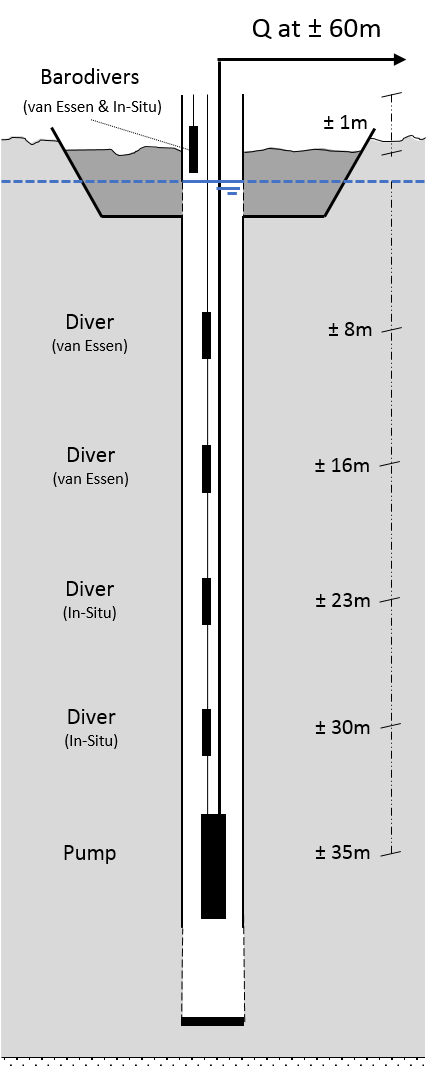
\includegraphics[width=0.65\linewidth]						{Setup_pumping_test.png}
		\captionsetup{justification=centering}		
		\caption{\label{fig:general}}
		\end{subfigure}%\hfill
	\begin{subfigure}[b]{0.4\linewidth}
        \centering\includegraphics[width=0.65\linewidth]						{Setup_pumping_test_bingo.png}
		\captionsetup{justification=centering}		
		\caption{\label{fig:simplified}}
		\end{subfigure}
	\captionsetup{justification=centering}	
	\caption{Fieldwork (measurement) set-up (\subref{fig:general}) general, ~(\subref{fig:simplified}) simplistic} 
	\label{fig:set-up}
\end{figure} 

Besides the divers, the measurement set-up also accommodates two baro-divers (van Essen \& In-Situ). The baro-divers are positioned in the borehole top section. Drawdown is by definition expressed as time dependent GWT reductions relative to the initial status. Short-term atmospheric fluctuations in pressure are compared to the water pressures negligible small. Nonetheless, these minor atmospheric influences are also included in the data collection. 
\bigskip \\
\textbf{Pumping test duration \& time measurement} \\
For each individual pumping test the exact start of pump operation could not be determined in advance. As a consequence, the total pumping test duration differs per pumping test as well. In every single measurement, a minimum of four hours of pumping and one hour of recovery is pursued. \\
To avoid unnecessary risks in missing out on the collection of drawdown data, all pressure sensors are programmed to start logging in time (08:00:00, local time, at pumping test days). All divers are set to log with a similar linear interval of 10 seconds. As a single exception, the In-Situ BaroTROLL is programmed to linear log once a minute (its minimum sample interval). \\

(* More detailed information on all equipment applied in fieldwork can be found in Appendix \ref{chapter:fieldwork_set-up}) 

\subsection{Data analysis}
\label{subsection:derivation_methods}
Raw drawdown time series are the result of fieldwork measurements. The data sets are more or less meaningless on its own. The methods below describe the required components in analysis to transforms the obtained fieldwork data to the desired transmissivity ($T$)and storativity ($S$) values. \\

\textbf{Simplified theoretical models} \\
The original borehole log sheets (appendix \ref{chapter:Borehole_logsheets}) are the most reliable source of local geological information available. Although the sheets contain site-specific information, similarities in stratification are present. In each case (\ref{section:research_locations}) the upper 50 m is divided into two or three layers, consisting of a (semi-)impermeable top layer and below that one or two high(er) permeable layers (aquifers). Groundwater tables are predominantly positioned slightly below the bottom of (semi-)impermeable layer, in the top aquifer (labelled as layer 1 in the figure below). Strictly seen, the conditions are therefore unconfined. But given the small interval (relative to total model thickness) between the the aquifer top and the GWT, the situation is close to confined. Based on the borehole log sheets three simplified theoretical models for the analysis of fieldwork data are proposed, as depicted in Figure \ref{fig:schematic_fieldwork_analysis}. 

\begin{figure}[h!]
	\centering
	\begin{subfigure}[b]{0.21\linewidth}
		\centering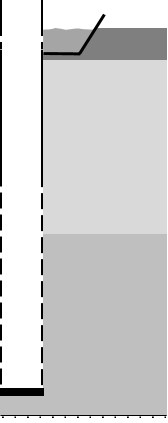
\includegraphics[width=0.6\linewidth]{Schematic_general_analysis}
		\captionsetup{justification=centering}		
		\caption{\label{fig:Schematic_general_analysis}}
		\end{subfigure}%\hfill
	\begin{subfigure}[b]{0.12\linewidth}
		\centering
\includegraphics[width=0.6\linewidth]{arrow_right}
		\end{subfigure}%\hfill
		%{\LARGE$\yrightarrow{}$}
	\begin{subfigure}[b]{0.21\linewidth}
		\centering
\includegraphics[width=0.6\linewidth]{Schematic_1lay_analysis}
		\captionsetup{justification=centering}		
		\caption{\label{fig:Schematic_1lay_analysis}}
		\end{subfigure}%\hfill
	\begin{subfigure}[b]{0.21\linewidth}
        \centering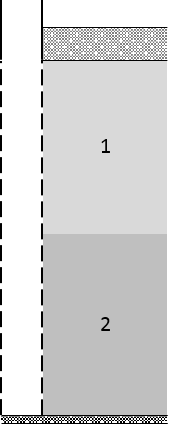
\includegraphics[width=0.6\linewidth]{Schematic_2lay_analysis}
		\captionsetup{justification=centering}		
		\caption{\label{fig:Schematic_2lay_analysis}}
		\end{subfigure}
	\begin{subfigure}[b]{0.21\linewidth}
        \centering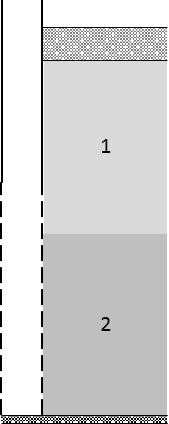
\includegraphics[width=0.6\linewidth]{Schematic_3lay_analysis}
		\captionsetup{justification=centering}		
		\caption{\label{fig:Schematic_3lay_analysis}}
		\end{subfigure}
	\captionsetup{justification=centering}	
	\caption{Schematic cross-sectional view of (\subref{fig:Schematic_general_analysis}) generalized northern Ghana soil stratification and simplified representations: (\subref{fig:Schematic_1lay_analysis}) a single layer system, ~(\subref{fig:Schematic_2lay_analysis}) a double layer system, and ~(\subref{fig:Schematic_3lay_analysis}) a system with two layers and partial penetration of the well} 
	\label{fig:schematic_fieldwork_analysis}
\end{figure} 

These simplified models (Figure \ref{fig:Schematic_1lay_analysis} - \ref{fig:Schematic_3lay_analysis}) mimic local conditions, making the derivation of representative hydraulic subsurface characteristics ($T$ and $S$) potentially possible \citep{Kruseman2000}. Double layered models are applied to provide more degrees of freedom, perhaps resulting in more accurate solutions. To limit the chances of equifinality (abundant degrees of freedom) a maximum of two soil layers are implemented in data analysis. \\ 

\textbf{Parameter derivation method's \& model environment} \\
It lacks a single best approach in the derivation of the geohydrological parameter values ($T$ and $S$). A widespread variety of analyses (e.g. analytical and computational) can be applied on the pumping test data. The details of the (analytical) models and methods used in this research are described below.

\begin{itemize}
\item{Theis's method} \\
Groundwater drawdown due to the withdrawal of water can be determined analytically with Theis's equation (Equation \ref{eq:theis}). Theis's method is applicable on the situation depicted in Figure  \ref{fig:Schematic_1lay_analysis}; a constant rate pumping test applied on a well that is fully penetrating a single layer aquifer \citep{Kruseman2000}. Confined conditions are assumed in Theis's method. Therefore, this analytical solution is suitable for obtaining a first indication (approximation) of the research geohydrological parameters.   
\end{itemize}


\begin{equation}
\label{eq:theis}
 s = \frac{Q}{4\pi K D} exp1(u)
\end{equation}

\begin{equation}
 u = \frac{r^{2} S}{4 K D t}
\end{equation}

Where $s$ (m) is the drawdown at distance $r$ (m) from the well, $Q$ (m$^{3}$) is the constant well discharge , $KD$ (m$^{2}$/d) is the aquifer transmissivity ($KD$ = $T$), $S$ (-) is the aquifer storativity, $t$ (d) is the time measured from the start of pumping and $exp1$ is the exponential integral. The drawdown measurements in this research are limited to in-well measurements. The distance $r$ in Theis's equation is assumed to be the length of the well radius (0.0635 m). Appendix \ref{sec:python_analysis} shows the implementation of Theis's method in Python.

\begin{itemize}
\item{Analytic Element Modelling in TTim} \\
TTim is a computer program based on analytic elements and designed for the analysis of transient groundwater flow. The analysis can be applied on a single or multiple layer(s). Several analytical elements (and types of elements) can be added to model layers. The use of TTim makes it possible to take additional well characteristics into account. Groundwater heads can be determined inside the well and the model optionally accounts for borehole storage and well skin resistance. Moreover, well discharge can be toggled on and off multiple times. This allows for simulations of both single pumping-recovery tests and long-term well operations \citep{Mishra2013,Bakker2013}. \\

This research fieldwork data is analysed within the TTim \texttt{Model3D} configuration. A single well (analytical element) is included in the model environment. The groundwater heads are determined inside the well. Aspects as actual borehole storage, optimal borehole storage and/or optimal well resistance are alternately accounted in different compositions of analysis. Moreover, the three types of simplified theoretical models (Figure \ref{fig:schematic_fieldwork_analysis}) are consecutively considered. A complete overview of all approaches in data analysis (25x) can be found in Appendix \ref{sec:data_analysis overview}. \\

The top layer (aquifer 1 in Figure \ref{fig:schematic_fieldwork_analysis}) is configured as being a phreatic layer. In other words, the top layer storage coefficient ($S$) is a phreatic storage coefficient ($S_y$). This model assumption is based on the observed initial groundwater tables, which are located below the bottom of the (semi-)impermeable top layer. In analysis, each simplified model layer has a hypothetical thickness of 1 m. The derived hydraulic conductivities ($k$) can therefore be interpreted as transmissivities ($T$) and the storage is expressed as the layer storage coefficient ($S$). This is done to directly derive $T$ and $S$ values. Additionally, this approach automatically corrects for the absence of knowledge on the thickness of the deepest soil layer in which the well is screened. There is no information about soil conditions beyond the bottom of the wells in the borehole log-sheets (Appendix \ref{chapter:Borehole_logsheets}). \\
\end{itemize} 

\textbf{Optimization functions} \\
As a final step in the determination of values for $T$ and $S$, the analytical solution (Theis's method) and composed TTim models are linked (fitted) to the fieldwork data. Two optimization functions are applied.

\begin{itemize}
\item{Fmin-RMSE function} \\
Differences between the measured and modelled drawdown (curves) can be expressed by the Root-Mean-Square-Error (RMSE) objective function (Equation \ref{eq:RMSE}). The \texttt{Fmin} function (part of Python's \texttt{scipy.optimize} package) is applied to minimize the RMSE value. In other words, the function is applied to minimize the difference between modelled and observed drawdowns. The optimization results in (RMSE based) optimal $T$ and $S$ values (and optionally values for borehole storage and/or well skin resistance). These values theoretically represent local conditions. An example Python implementation of the \texttt{Fmin-RMSE} optimization function is depicted in Appendix \ref{sec:python_analysis}. 
\end{itemize}
% example of monospace use: \texttt{hier wat je wilt hebben in monospace}!

\begin{equation}
\label{eq:RMSE}
 RMSE = \sqrt{\Sigma\frac{(s_{mod}-s_{field})^{2}}{N}}
\end{equation}

Where $s_{\text{mod}}$ is the modelled drawdown (m), $s_{\text{field}}$ is the observed drawdown (m) and N is the number of data points. \\
 
\begin{itemize}
\item{Calibration function} \\
TTim has an in-built calibration function for the derivation of parameter values. Application of this second method improves the research robustness (reference values). An example of the Python implemented TTim \texttt{Calibrate} optimization function is part of Appendix \ref{sec:python_analysis}. \\
\end{itemize}

Both optimization methods require initial parameter estimations. More than one suitable solution is possible, which makes the outcome of the optimization dependent on the choice of the initial values. Other studies found that $T$ and $S$ values are commonly low in northern Ghana \citep[e.g.][]{Owusu2015,Owusu2017}. Based on these other studies the following initial conditions are applied: $k_{aq0}$ is 10 (m/d), $k_{aq1}$ is 10 (m/d), $S_{aq0}$ is 0.01 (-), $S_{aq1}$ is 0.001 (-) and well resistance is 0.1 (d). The well radius (measured in-field) is used as the (initial) borehole storage: 0.0635 (m). Boundary conditions are applied to avoid the optimization resulting in physically improbable parameter values, i.e. negative parameter values and unnaturally high storativity values (greater than 0.3 (-)).

%(write something over initial conditions. Such small values. Not one single best solution. multiple 'best' solutions potentially close to each other. so solutions highly influential by the arbitrary chosen initial conditions. For each location several attempts done to see which initial conditions score pretty good. And subsequently generalization of those initial parameters applied per location/pumping test. for example better fit at Bingo at initial condition for T (KD) of 10, 10 (lay one and two) for fmin then for cal (2 layered system.) But 2 layered system all of sudden scores better with initial conditions 5, 1 for example.  

\section{Methods - ASR system improvements}
\label{section:test_problem_def}
A hypothetical northern Ghana test problem is selected to explore and access the capabilities of a locally applicable ASR system. The natural conditions are simplified and represented in a synthetic model. The applied model representation of nature is defined in this part of the research methodology. The section contains information on; the base model (reference), the types of ASR system improvement/sensitivity and the test criteria applied in research. The results are elaborated in Chapter \ref{chapter:model_scenarios}. Additional information on the modelling environment (MODFLOW) is included in the Appendices \ref{chapter:Extense_Modflow_model} - \ref{MODFLOW_radial}. 

%General aim of research is pointed at the provision of larger water quantities during northern Ghana's dry seasons. The research investigates to what extent Aquifer Storage and Recovery systems (ASR-systems) can contribute to water availability. The water is in the essence used for local small-scale agriculture. \\
%
%in ASR-system improvements upscaling. The test problem consists of a single layer aquifer which is partially penetrated by a well. In accordance with \citet{HoughtonMifflin2016}, upscaling can be defined as \emph{"The raise to an higher level; an upgrade"}. Free interpretation learn, multiple directions of upscaling are applicable. The single test problem is exposed to three types of ASR-system upscaling; (1) upscaling in dry season daily pumping time, (2) upscaling the borehole cross-sectional dimension and (3) upscaling by ASR-system cleaning. \\
%
%The hypothetical northern Ghana test problem will be outlined first. It concerns both the natural (Section \ref{section:test_problem_def}) as well as the model-based description (Section \ref{section:MODFLOW_const}). As a follow-up, the unimproved (base) model performance is described (Section \ref{section:Base_model_perf}). The section can be used as reference material for the different types of system upscaling (Section \ref{section:ASR_upscaling}). The chapter concludes with a discussion on the (ASR-system upscaling) results obtained (Section \ref{section:Upscaling_conclusions}). 

\subsection{Synthetic base model definition (reference)} 
\label{base_model_def}
The research is provided with an ASR system base model. Unsurprisingly, the base model accommodates basic conditions. The conditions applied are based on northern Ghana fieldwork and the gathered borehole log sheets (Appendix \ref{chapter:Borehole_logsheets}). The simplified model represents a fictive 'standard' ASR system, potentially applicable in northern Ghana. The base model is a reference, a starting point to which the impact of system improvements can be compared. The distinctive system component (e.g. well characteristics and time frame) are one-by-one described here. The overall representation of the base model is depicted in Figure \ref{fig:Schematic_base_model_empty}. \\

\tikzstyle{mybox} = [draw=black, fill=white, very thick,
    rectangle, rounded corners, inner sep=20pt, inner ysep=20pt]
\tikzstyle{title} =[fill=black, text=white]

\begin{figure}[h]
\centering
\begin{tikzpicture}
\node [mybox] (box){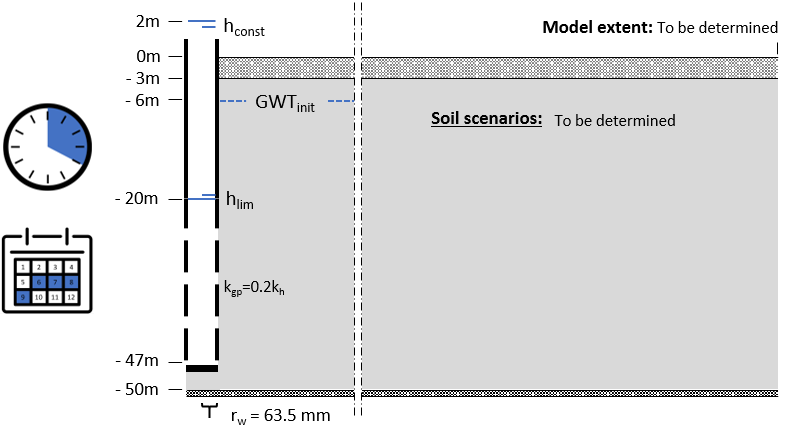
\includegraphics[width=0.7\linewidth]{Schematic_base_model_empty}};  
\node[title, right=10pt] at (box.north west) {Schematic base model (reference)};
\end{tikzpicture}
\captionsetup{justification=centering}
\caption{Schematic base model (reference)}
\label{fig:Schematic_base_model_empty}
\end{figure}

\textbf{Soil scenarios} \\
The interaction between the ASR-system and the upper 50 m of subsurface is simulated. The model top is bounded by a 3m-thick poor permeable soil layer. Well penetration occurs in the underlying 47m-thick aquifer(s). With an elevation of -6 m the initial groundwater table (GWT) is positioned just under the aquifer top. Unconfined conditions are applicable. The aquifer is assumed to be homogeneous and horizontally isotropic, while the vertical anisotropy is 1/4 (-). The results of the fieldwork data analysis (characteristic $T$ and $S$ values for one or more layer(s), determined in Chapter \ref{chapter:Fieldwork_data_analysis}) are stated to be used as input for the definition of (multiple) soil scenarios. The exact applied soil scenarios are defined at the start of Chapter \ref{chapter:model_scenarios}. Subsequently, the model extent (radial distance from well) is based on these outcomes. More information on the definition of the radial extent can be found in Appendix \ref{section:Leakage_factor}.\\

\textbf{Well dimensions \& pump placement} \\
The base model design accommodates a single well with a radius of 0.0635 m (2.5 inch) and a total length of 47 m. It is assumed, in-well accumulation of sedimentation is absent. The displacement of water between well and aquifer is possible through a partially penetrating screen. Well screen perforation are present from 20 m to 47 m below the model top (screen length 27 m). More details on the well hydraulic conductivity can be found below. Dry season groundwater withdrawal is possible through the installation of a pump. The model contains a pump at an elevation of -30 m. The maximum drop in GWT is limited to an elevation of -20 m (14 m drawdown relative to initial conditions). In this way the occurrence of well screen dry-out and pump malfunctioning is prevented. \\

\textbf{Well hydraulic conductivity} \\
Due to the tiny nature of screen perforations (and constructional soil around the borehole), a well skin hydraulic conductance / resistance is taken into account. In this research the well hydraulic conductance is defined by the use of Equation \ref{eq:cond} - \ref{eq:K_skin}. 

\begin{equation}
 cond = \frac{2\pi r_w b}{c_{skin}}
\label{eq:cond}
\end{equation}

\begin{equation}
 c_{skin} = \frac{\Delta r_{skin}}{K_{skin}}
\label{eq:c_skin}
\end{equation}

where $cond$ (m$^2$/d) is the well hydraulic conductance, $r_w$ (m) is the radius of the well, $c_{skin}$ (d) is the well skin resistance , $\Delta r_{skin}$ (m) is the well skin length and $K_{skin}$ (m/d) is the well skin hydraulic conductance. \\

As stated by \citet{Houben2015}, the hydraulic conductivity of a sequence of materials (i.e. well screen, gravel-pack and aquifer) can be calculated by Equation \ref{eq:K_tot} (1D flow assumed). The model well cells are in this research defined in correspondence with the (radial) well dimensions. Therefore, the well skin conductance is assumed to be only dependent on the materials of the well screen and the gravel-pack. In this case, the well skin hydraulic conductivity corresponds with the simplified variant of Equation \ref{eq:K_tot}; Equation \ref{eq:K_skin}.  

\begin{equation}
 K_{tot} = \frac{\Delta r_{tot}}{\frac{\Delta r_{sc}}{K_{sc}} + \frac{\Delta r_{gp}}{K_{gp}} + \frac{\Delta r_{aq}}{K_{aq}}}
\label{eq:K_tot}
\end{equation}

\begin{equation}
 K_{skin} = \frac{\Delta r_{skin}}{\frac{\Delta r_{sc}}{K_{sc}} + \frac{\Delta r_{gp}}{K_{gp}}}
\label{eq:K_skin}
\end{equation}

where $K_{tot}$, $K_{skin}$, $K_{sc}$, $K_{gp}$ and $K_{aq}$ (m/d) are respectively the total, the well skin, the well screen, the gravel-pack and the aquifer hydraulic conductivities and ${\Delta r_{tot}}$, ${\Delta r_{sc}}$, ${\Delta r_{gp}}$, ${\Delta r_{aq}}$ (m) are the corresponding length intervals of these materials. \\

The length of the well skin ($\Delta r_{skin}$) is the sum of the well screen ${\Delta r_{sc}}$ and the gravel-pack ${\Delta r_{gp}}$ length. Based on fieldwork measurements, a well screen length of 0.005 m is used. The radius of the soil around the well, the gravel-pack, is unknown. As stated by \citep{Bot2016}, for proper installation a minimum length of 0,125 m is required. This length is assumed and implemented in research. \\

The well skin hydraulic conductivity ($K_{skin}$) accounts for the combined conductivity of the well screen (perforations) and the gravel-pack around the well. The hydraulic conductivity of the well screen ($K_{sc}$) is based on research done by \citet{Houben2015}. Perforation sizes (screen slot width) of 2 mm are measured (fieldwork). These screen sizes correspond with a (clean) hydraulic conductivity ($K_{sc}$) of 1 m/s \citep{Houben2015}. In general, $K_{skin}$ values are typically expected to be lower than the $K_{h}$ \citep{LeonardF.KonikowGeorgeZ.HornbergerKeithJ.Halford2009}. To meet this requirement, the gravel-pack is interpreted as partially clogged. The research base model $K_{gp}$ is assumed to be 1/5 of the $K_{h}$ (soil scenario dependent). \\

%(Equation \ref{eq:cond}). The well skin resistance ($c_{skin}$) is inversely proportional to the well skin hydraulic conductivity ($K_{skin}$). The well skin hydraulic conductivity is typically lower than the original aquifer hydraulic conductivity ($K_{h}$)  \citep{LeonardF.KonikowGeorgeZ.HornbergerKeithJ.Halford2009,Houben2015}. A base model well skin hydraulic conductivity that equal 1/5 of the aquifer hydraulic conductivity is assumed. The definition of the well skin resistance is detailed described in


\textbf{Time frame} \\
As stated by the \citet{HAP2011}, on a yearly basis northern Ghana encounters a single wet season of approximate four months (dependent on the year and altitude). Randomly applied interviews with local inhabitants (fieldwork) confirmed the temporal resolution of the wet season. During wet season inundation levels of 0.5 m - 4 m are perceived, with a timespan varying from weeks till the (four months) duration of the wet season. \\
Seasonal system behaviour is simulated by a year-round (long term) temporal model resolution. In the synthetic (simplified) model it is assumed the region encounters flooding for as long as the wet season. A flooding for the duration of four months, starting on June 1$^{st}$ and ending on September 30$^{th}$. The flooding is simulated by gravity based infiltration on top of the ASR system. A constant (122 days) 2 m inundation level is assumed (Figure \ref{fig:Schematic_base_model}). In the subsequent eight months of dry season (October-May) no flooding or rainfall is taken into account. In accordance with interview outcomes, groundwater withdrawal takes place by four hours of pumping daily. Intermediate day time offers time-space for GWT recovery. For the purposes of this research it is assumed the hypothetical groundwater withdrawal last for as long as the dry season (243 days). \\

%These results are determined in subsequent parts of research (Chapter ). As a follow-up, the soil sceanrios applied in simulation are Chapter \ref{}  the or the  bandwidth of transmissivity and storativity values (derivatives from fieldwork data analysis (Chapter \ref{Fieldwork_data_analysis})), is used for the definition of five aquifer scenarios. An overview of the applied scenarios can be found in Figure \ref{fig:Schematic_base_model}).  These conditions are the base for the simulation of unsteady state flow in the radial and vertical direction.

\textbf{Model discussion} \\
The research base model results do not apply to a single research location (depicted in Figure \ref{fig:Overviewlocations}). The applied simplified model conditions serve research purposes. Assumptions made, are not by definition realistic. One can for example imagine the actual wet season inundation levels will fluctuate over time. And in practice, groundwater withdrawal needs day-specific tuning (not constant for 243 days) with respect to agricultural needs. Aspects advisable to take into account in further research.\\

%Obtained results should only be interpreted as indicative (improvement) options in northern Ghana ASR-system application. 

\textbf{Modelling environment - MODFLOW} \\
The computational modelling of the base model (and the ASR system improvements) is done with Modular Ground-Water Flow Model (MODFLOW), a finite difference model for groundwater flow developed by the U.S. Geological Survey (USGS). MODFLOW is the international standard in groundwater simulation \citep{Niswonger2011,HarbaughArlen2005}. More information on the applied inputs can be found in the Appendices \ref{chapter:Extense_Modflow_model} - \ref{MODFLOW_radial}.

%In the case of fieldwork data analysis  MODFLOW is not used for the derivation of geohydrological parameters. Optimal parameters derived with TTim models are implemented in corresponding MODFLOW models to validate obtained TTim results. More information on the modelling part can be found in Appendix.

\subsection{ASR system improvements}
\label{subsec:improvements}
A free interpretation of the term 'improvement' learns that multiple directions of ASR system modifications are applicable. As stated by \citet{Bakker2010} and \citet{Ward2007}, the success and sustainability of an ASR system is amongst others dependent on the length of injection, storage and recovery; the well dimension; and potential clogging of the well screen. The synthetic model of this research is exposed to three related types of ASR system improvement:

\begin{itemize}
\item{a) Extension of daily pumping time:} \\
In a consecutive order the base model dry season pumping time (4 hours daily) is increased (by 1 hour steps) up to a maximum daily (dry season) pump operation of 8 hours.
\item{b) Enlargement of borehole cross-sectional dimension:} \\
The base model radius (0.0635m) is stepped up (doubled, tripled, etcetera) to in total five times its original radius: 0.3175 m. 
\item{c) Reduction of well skin resistance:} \\
This type of synthetic model improvement is designed by the application of enlarged gravel-pack hydraulic conductivities. In four equal steps (steps of (2/5)*$K_{h}$) the base model gravel-pack hydraulic conductivity ($K_{gp}$) is increased to a maximum of (9/5)*$K_{h}$. Note; well skin hydraulic conductivities larger than the aquifer hydraulic conductivities are considered in this way. More information on the calculation of the well skin conductance / resistance is stated in the Equations \ref{eq:cond} - \ref{eq:K_skin}.
\end{itemize}

\subsection{ASR system sensitivities}
\label{subsec:sensitivity}
The forces of northern Ghana's nature can highly fluctuate spatially and temporarily. Nonetheless, the base model houses multiple assumptions that are more or less fixed representations of nature (\ref{base_model_def}). A sensitivity analysis is part of the research to balance the impact of these assumptions. Three types of model modifications are part of the sensitivity analysis: 

\begin{itemize}
\item{a) Degradation of well depth (clogging):} \\
The fieldwork observations imply that ASR systems in northern Ghana can be vulnerable for the power of nature. Due to the accumulation of sedimentation the well penetrations depths can decrease over time. The reduction is simulated by a decrease in the well screen length. An hypothetical initial screen length of 30 m is reduced (steps of 5 m) to 10 m.
\item{b) Shortening the wet season inundation timespan:} \\
The impact of lower inundation levels is analysed in combination with increased initial groundwater tables. Relative to the base model ($\Delta h$ is 8m) the $\Delta h$ is reduced (in steps of 2 m) to a minimum of $\Delta h$ is 2 m.   

\item{c) Reduction of wet season inundation level:} \\
The impact of lower inundation levels is analysed in combination with increased initial groundwater tables. Relative to the base model ($\Delta h$ is 8m) the $\Delta h$ is reduced (in steps of 2 m) to a minimum of $\Delta h$ is 2 m.   
\end{itemize}

%\begin{itemize}
%\item{a) Degradation of well depth (clogging):} \\
%The fieldwork observations imply that ASR systems in northern Ghana can be vulnerable for the power of nature. Due to the accumulation of sedimentation the well penetrations depths can decrease over time. The reduction is simulated by a decrease in the well screen length. An hypothetical initial screen length of 30 m is reduced (steps of 5 m) to 10 m.
%\item{b) Shortening the wet season inundation timespan:} \\
%Within northern Ghana the duration of the wet season is spatially dependent \citep{HAP2011}. Besides, season durations naturally differ between years. Through the application of three steps the synthetic base model wet season duration is reduced from four months till one.
%\item{c) Reduction of wet season inundation level:} \\
%Different flood inundation levels are encountered by local inhabitants. As mentioned by the \citet{HAP2011}, wet season intensities vary within northern Ghana. Besides, initial groundwater tables are not fixed. Based on the fieldwork inspection it is confirmed that the GWT in northern Ghana varies. The impact of lower inundation levels is analysed in combination with increased initial groundwater tables. Relative to the base model ($\Delta h$ is 8m) the $\Delta h$ is reduced (in steps of 2 m) to a minimum of $\Delta h$ is 2 m.   
%\end{itemize}

%At all study site locations (\ref{section:research_locations} measured borehole depths are less than original. The accumulation of sedimentation reduces the active borehole depth over time.  the borehole depth decreases due to the (e.g. ASR system location Nungo)   bldednhecnecdnennenqcnnencncbbcecbcbcbcjbcbcjcj

\subsection{Test criteria - sustainability}
As mentioned in Section \ref{base_model_def}, synthetic model performance is simulated in the time frame of a year. A distinction can be made between the wet and dry season. The wet season ASR-system behaviour is characterized by the inflow of water. Analysis is pointed at the volumes recharged and the impact of these volumes on GWT. In the subsequent eight months of dry season, the system works in reverse. In this time of year, maximum pump operation and the accompanied impact on GWT is of key interest. \\
As a supplement, the mutual relation between in- and outflow is considered. This is done by the introduction of the 'Recovery Ratio' $R_{\%}$ (Equation \ref{eq:RR}). The Recovery Ratio is similar to Recovery Efficiency (RE) applied by \citet{Ward2007}. The RE ($R_{\%}$) is a measure to indicate the degree of recovery, i.e. RE = 1 (-) (100\%) implies complete recovery \citep{Ward2007}. 

\begin{equation}
 R_{\%} = \frac{V_{out,tot}}{V_{in,tot}}
\label{eq:RR}
\end{equation}

Where  R$_{\%}$ is the year-round Recovery Ratio (-), $V_{in,tot}$ (m$^3$) is the wet season total volume recharged and $V_{out,tot}$ (m$^3$) is the dry season total volume discharged. \\

The system sustainability is discussed through the recovery ratio. A $R_{\%}$ smaller than 1 (-) indicate a year round net inflow. In this case, the interaction between system and nature is positive. For the purposes of this research 'sustainability' is defined as a situation where the $R_{\%}$ is smaller than or equal to 1 (-). The potential increase in groundwater withdrawal, due to synthetic improvements, is limited by sustainability. In other words, a 100\% recovery is set as an upper boundary to guarantee sustainability. 

\section{Methods - ASR system financial yield}
\label{section:Theory_yields}

The performances of Aquifer Storage and Recovery systems (ASR-systems) are generally expressed in water volumes. The volumetric results are desirable, but it is hard to get a good picture of it. Some simplistic transformations make it possible to express the obtained volumes in agricultural and financial yield.  This part of the methodology facilitates a glimpse in the northern Ghana ASR system (financial) feasibility. The system yield is expressed by the definition of specific crops of interest. The yield is weighted against the water withdrawal pumping costs.
%An rough insight is given by weighing (crop specfitc First, an explanation on applied theories in transition from water volumes to agricultural field-sizes and financial yields (Section \ref{section:Theory_yields}). Subsequently the previously obtained water volumes are exposed to the transformation (Section \ref{section:Data_processing}). This part of research ends with a conclusive remark on ASR-system yields and posibilities in spatial multiplication (Section \ref{section:Yields_conclusions}). 

\subsection{Yield - crops of interest}
Some crops need more water than others. Some crops thrive better in northern Ghana climate than other. Some crops are financially more beneficial than others. And so, many more elements are decisive in the process of crop type determination. This research is not about crop type decisions. The crops (mentioned below) are purely included in the study to gain knowledge on hand-on possibilities in the agricultural use and financial feasibility of ASR-systems in northern Ghana. \\
%Keeping northern Ghana applicability in mind a selection of crops is made. 

\textbf{Crops of interest}
\begin{itemize}
\item{Tomato} \\
The worldwide second most important vegetable crop (after the potato) concerns the tomato. Because of its relative high (financial) yield, the vegetable is a desired crop for cultivation. After a period of approximately 90 to 120 days the seeds are grown to fully-fledged crops, the tomatoes are ready for harvesting. Over the growth season the crop thrives best by the supply of 400 to 600 mm of water (rain-fed). To reduce the chances of deceases (pests and infestations) the crop should be cultivated in rotation with other crops. Under the conditions of irrigation the tomato yield is approximately 45 to 65 ton/ha \citep{FAO2018a}. Because of the broad ranges in agricultural yield and water requirements (moreover, only rain-fed statistics), these specific crop competences are not taken into account in research. The derivation of agricultural yield is based on the average 'water utilization efficiency' ($E_y$). For the transformation of agricultural yield to financial benefits, the Esoko march 2018 Ghana average wholesale price is used. The tomato wholesale price is set at a value ranging from 217.86 to 220.43 GHS for a 52 kg crate \citep{ModernGhana2018}. For the purposes of this research the highest average value is applied. To summarize: 
\begin{itemize}
\item{Length growth season: 120 (d)}
\item{Water utilization efficiency: $E_y$ = 11 (kg/m$^3$)}
\item{Wholesale price: 4.239 (GHS/kg)}
\end{itemize}

\item{Groundnut} \\
The groundnut is an above average profitable crop grown in Ghana. Production is often the responsibility of small holder farmers in the North. Almost the complete Ghana groundnut production originates here \citep{Ghana-made2018}. Growth season length is dependent on the varieties (sequential or alternately). In general harvesting can take place after a period of 90 to 140 days. For a proper single season production, groundnut crops require approximately 500 to 700 mm of water. Rain-fed crops can produce average yields of 2-3 ton/ha unshelled nuts. By the introduction of irrigation these values even reach 3.5-4.5 ton/ha \citep{FoodandAgriculturalOrganisationoftheUnitedNationsFAO2018a}.  At the contrary, a 2016 Ghana average agricultural yield of 1.25 ton/ha unshelled groundnut is perceived \citep{FoodandAgriculturalOrganisationoftheUnitedNationsFAO2018}. 
In other words, groundnut crop yield are not unambiguous. The \citet{FoodandAgriculturalOrganisationoftheUnitedNationsFAO2018a} average water utilization efficiency ($E_y$) is adapted as normative. Financial yields are highly fluctuating over time. Market forces are dominant in actual returns. The march Esoko 2018 Ghana average unshelled groundnut wholesale price is set at a value ranging from 247.50 to 282.50 GHS for a 82 kg bag \citep{ModernGhana2018}. For the purposes of this research the highest average value is applied and interpreted as the unshelled groundnut price. To summarize:
\begin{itemize}
\item{Length growth season: 123 (d)}
\item{Water utilization efficiency: $E_y$ = 0.7 (kg/m$^3$)}
\item{Wholesale price: 3.445 (GHS/kg)}
\end{itemize} 
\end{itemize}

As stated before, the time frame of the synthetic simulation consist of 243 days of dry season. It is assumed two consecutive growth seasons fit this period. The tomato growth season is succeeded by a growth season labelled for the production of groundnut. This complies with the desire of rotational crop cultivation. \\

The applied crop specifications are dominated by supreme rough assumptions in e.g. quantity (kg) and prices. The obtained (financial) yields should solely be interpreted as indicative. In other words, "All rights reserved". \\
 
\textbf{Irrigation efficiency} \\
The dry season agriculture is assumed to be purely dependent on irrigation for the supply of water. Different types of irrigation are suitable in northern Ghana. One can think of border strip/furrow irrigation; simplistic but inefficient. Higher degrees of efficiency can be achieved by the use of sprinkler irrigation. In the particular case of ASR-system use, minimum water losses are pursued. Therefore, drip irrigation is applied. Drip irrigation is the type of irrigation with the highest efficiencies. Systems are standard paired with facilities as poly-tank(s), pipes and drip hoses. Distances between extraction and irrigation are small, resulting in limited losses. However, water losses are present due to pipe connections and potential evaporation. All-encompassing, a irrigation system efficiency of 0.8 (-) is considered. 80\% of all water withdrawn is assumed to be net usable for crop growth \citep{VandeGiesen2013}. Note, this efficiency number also accounts for the in practice required schedule in irrigation water amounts. Over the growth season the required water volumes are here  hypothetical and assumed to be daily equal. \\
%
%\textbf{Cover area (crop specific)} \\
%Water volumes obtained in previous research sections are basic input for the determination of agricultural field sizes. Net withdrawn (dry season) total volumes are divided by the crop specific water footprint. The areal outcome is halved to correct for the double (consecutive) growth periods in a single dry season.   
%
%\begin{equation}
% A = \frac{V_{out,tot} * \eta_{irrigation}}{2 * Water footprint_{crop}} 
%\label{eq:A}
%\end{equation}
%
%Where, A (m$^2$) is the agricultural field area, $V_{out,tot}$ (m$^3$) is the dry season total volume discharged, $\eta_{irrigation}$ (-) is the irrigation efficiency and $Water footprint_{crop}$ (m) is the crop specific water footprint. \\
%
%The extraction of water leaves marks on nature. Pump operation causes a groundwater cone of depression. Close range (and most definitely in-well) drawdown is significant. At an increased radial distance impact losses magnitude. For system spatial multiplication it is of interest to define a maximum circular area in-which groundwater is affected. The groundwater cone of influence (G) is defined as the area corresponding with the maximum radius from well at which the groundwater drawdown is labelled as significant. In this study, significance is assumed to be bounded by a drawdown of 1.0 m at any moment in year. \\
%
%\begin{figure}[h]
% \centering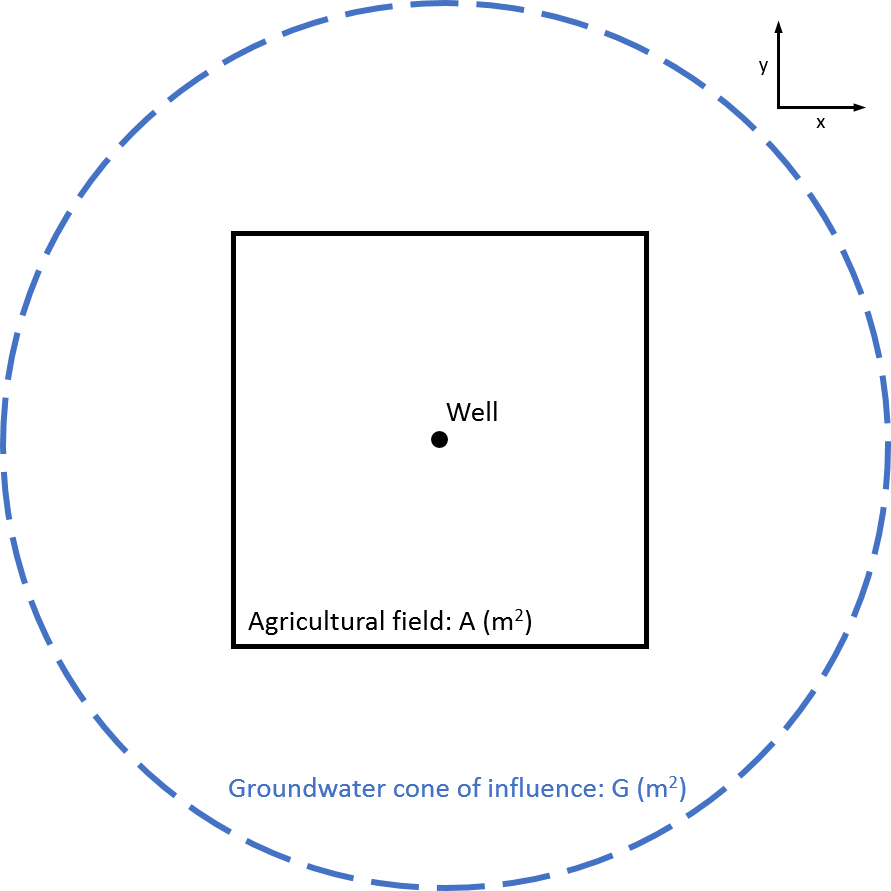
\includegraphics[width=0.4\linewidth]{Crop_cover}
% \captionsetup{justification=centering}
% \caption{Fictive schematic of crop cover area (C$_\%$)}
% \label{fig:Crop_cover}
%\end{figure}
%
%The A over G ratio ($C_{\%}$) shows top-view perspectives of spatially concatenated multiplication of agricultural fields, as visualized in Figure (\ref{fig:Crop_cover}). High $C_{\%}$ values (close to one) suggest the implementation of agricultural fields is possible at close mutual distance. \\
%
%\begin{equation}
% C_{\%} = \frac{A}{G}
%\label{eq:RR}
%\end{equation}
%
%Where  C$_{\%}$ is the crop cover ratio (-), $A$ (m$^2$) is the crop specific agricultural field size and $G$ (m$^2$) is the areal groundwater cone of influence. \\

\textbf{Financial yield} \\
Based on the described crop specification, the simulated water volumes withdrawn can be expressed in financial returns. The agricultural yield (kg/m$^3$) and the weighted crop prices (GHS/kg) are defined. From consistence considerations it is chosen to express the financial returns in US dollars. The July 7$th$ Bloomberg financial exchange rate is applied: 0.2081 USD/GHS \citep{Bloomberg2018}.

\subsection{Costs - water withdrawal}
Profits are accompanied by costs. For this research all Capital Expenditures(CAPEX) are unknown and ignored. The same applies for large parts of the Operating Expenses (OPEX), e.g. farmer wage and fertilizer costs. The only costs accounted are related to the energy (diesel) consumption. Outcomes are purely focused on the feasibility of the daily system operation. An impression is generated, whether or not regular ASR-system operation on its own is profitable. \\

\textbf{Synthetic pump application} \\
The Pedrollo 4" submergence pump is applied in fieldwork measurements. The same pump, i.e. its specifications, is used a standard in the subsequent parts of research. General specification can be found in Appendix \ref{chapter:Pedrollo_product_specs}. The results of the synthetic simulations contains time dependent (4 hours daily, 243 days) discharge rates. As soon as the maximum pumping capacity is exceeded, it is assumed the specific simulation is carried out by the implementation of an extra (same) pump. By a parallel pump configuration the same heads and efficiencies are ensured, while discharge capacities are doubled \citep{VandeGiesen2013}. \\ 
%As soon as the maximum pumping capacity is exceeded by the obtained (simulated) discharge rates (results Chapter \ref{chapter:model_scenarios}),

\textbf{Energy Consumption} \\
The available groundwater has to be lifted to the surface. Depends on the obtained discharges, the lifting action requires a certain magnitude of power (Equation \ref{N_net}). For water displacement the difference between pump position and surface level (30m) is retained. An extra lift of 15 m is added to account for friction losses and the higher position (above surface) of the poly tank(s). A total head lift of 45 m is applied.

\begin{equation}
N_{net} =  g * Q * \Delta H
\label{N_net}
\end{equation}

Where $N_{net}$ (kW) is the net power required, g (m/s$^2$) is the gravitational acceleration (9.81 m/s$^2$), Q (m$^3$/s) is the discharge (total extracted volume of water over the yearly sum of pumping time (in seconds)) and $\Delta$H (m) is the net head (total lift) required. In this equation it is assumed the water has a density of 1000 kg/m$^3$. \\

In general, the use of power gets accompanied by losses (for example due to friction and turbulence). Ever single power-related equipment works at a certain level of efficiency. The power generator applied in fieldwork (Appendix \ref{chapter:fieldwork_set-up}) is used over years. Due to its datedness, a generator efficiency of 70\% is estimated. The efficiency of the Pedrollo pump(s) is dependent on the discharge rate. An overview of the efficiency curve is present in Appendix \ref{chapter:Pedrollo_product_specs}. In this study, the pump efficiencies are related to the time dependent discharges obtained in the synthetic model simulations. Besides equipment losses, energy get lost due to mutual transmission. An extra efficiency value of 90\% is accounted \citep{VandeGiesen2013}. Result is a variable ASR-system efficiency of that never exceeds 36.5 \% (based on maximum pump efficiency).

\begin{equation}
 \eta_{total} =   \eta_{generator} * \eta_{transmission} * \eta_{pump} \end{equation}

Where $\eta_{total}$ (-) is the overall power efficiency, $\eta_{generator}$ (-) is the generator power efficiency, $\eta_{transmission}$ (-) is the transmission power efficiency and $\eta_{pump}$ (-) is the pump power efficiency. \\

The combination of total ASR-system efficiency and net required power results in a gross power \ref{Eq:gross}. The gross power should be delivered by the generator to gain the desired volumes of water at the agricultural fields. Multiplying the gross power required by the total hours of pump operation returns the total energy consumed (kWh).

\begin{equation}
 N_{gross} =   \frac{N_{net}}{\eta_{total}}
\label{Eq:gross}
\end{equation}

Where $N_{gross}$ (kW) is the gross power required, $N_{net}$ (kW) is the net power required and $\eta_{total}$ (-) is the overall power efficiency. \\

\textbf{Energy costs} \\
The Kipor power generator (Appendix \ref{chapter:fieldwork_set-up}) contains a 15 litre diesel tank. On a full tank the generator can operate for 6.5 hours. A fuel consumption of 2.31 l/h is taken into account. During operation the generator delivers a continuous power capacity of 4.5 kW \citep{TS242018}. Ghana diesel price of 5.03 GHS/l (begin of July) is adopted as normative \citep{GlobalPetrolPrices2018}. The Bloomberg financial exchange rate (0.2081 USD/GHS) is once again applied on the fuel costs for proper comparison with the agricultural yield \citep{Bloomberg2018}.

\begin{equation}
 Cost_{fuel} =  \frac{consump_{gen} * price_{fuel} * rate_{exchange}}{power_{gen}}
\end{equation}

Where $Cost_{fuel}$ (USD/kWh) is the price of fuel,  $consump_{gen}$ (l/h) is the generator fuel consumption,  $price_{fuel}$ (GHS/l) is the fuel price in Ghana, $rate_{exchange}$ (USD/GHS) is the Bloomberg financial currency rate and $power_{gen}$ (kW) is the generator continuous power capacity. 

